\documentclass[12pt, legalpaper]{article}
% 10pt es el tamaño de letra por default
% para modificarlo desde documentclass, solo permite 10pt, 11pt y 12. 
% Prueba comentario
\usepackage{graphicx} % Required for inserting images
\usepackage{float} % Se utiliza para el posicionamiento forzado de los elementos del documento (figuras y tablas)
\usepackage{subcaption} %mozaico de figuras
\usepackage{pdflscape}

\title{\Huge{Tiro con arco}}
\author{\small{Miguel Carrillo}}
\date{30 de Enero 2025}


\begin{document}

\maketitle

\section{\LARGE{Introducción}}

Elaboración de mi \textbf{primer} \emph{documento} para visualizar las opciones del tipo de \texttt{documento}. 

El tiro con \huge{arco} es un deporte en el que los participantes disparan flechas usando un arco con el objetivo de alcanzar una diana o blanco lo más cerca posible del centro. La \large{precisión} es clave, y cada disparo es puntuado según la cercanía al centro de la diana. En la figura \ref{tiro1}, se muestra una foto de un competidor.

\begin{figure}[H]
    \centering
    \includegraphics[scale=.1]{../../../../Downloads/THC_2025_2/diana.jpg} 
    \caption{Imagen ilustrativa del tiro con arco.}
    \label{tiro1}
\end{figure}

El tiro con arco es una práctica 'antigua' que comenzó como una técnica de caza y en la guerra. Sin embargo, como deporte organizado.
Corea del Sur domina este deporte a nivel olímpico. Han ganado más de 40 medallas (incluyendo alrededor de 27 de oro) desde que se reintrodujo en 1972. El éxito de Corea del Sur se atribuye a su sistema de entrenamiento riguroso y a la enorme popularidad del deporte en el país. 
%La probabilidad de que ganen los jefes de Kansas City es del 50\%.

\section{Mozaico de figuras}

A continuación se muestran los accesorios del tiro con arco. Por ejemplo, en la figura \ref{a} son las flechas y en la figura \ref{b} se observa la diana

\begin{figure}[H] % primeras dos subfiguras
    \begin{subfigure}{0.45\textwidth}
        \centering
        \includegraphics[scale=.1]{../../../../Downloads/THC_2025_2/diana.jpg} 
        %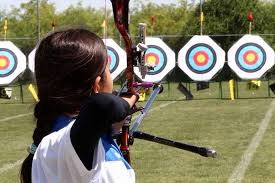
\includegraphics[scale=.35,angle=0]{imagenes/tiro_arco.jpg}
        \caption{Flechas}
        \label{a}
    \end{subfigure}
    \begin{subfigure}{0.45\textwidth}
        \centering
        \includegraphics[scale=.1]{../../../../Downloads/THC_2025_2/diana.jpg} 
        \caption{Soporte}
        \label{b}
    \end{subfigure} 
    
    \begin{subfigure}{0.45\textwidth} % otras dos subfigura
        \centering
        \includegraphics[scale=.1]{../../../../Downloads/THC_2025_2/diana.jpg} 
        \caption{Visor}
        \label{c}
    \end{subfigure}
    \begin{subfigure}{0.45\textwidth}
        \centering
        \includegraphics[scale=.1]{../../../../Downloads/THC_2025_2/diana.jpg} 
        \caption{Arco}
        \label{c}
    \end{subfigure}
    \caption{Accesorios del tiro con arco.}
\end{figure}

\subsection{Más figuras}

\newpage

\begin{landscape}
    \begin{figure}[H]
        \centering
        \includegraphics[scale=.15]{../../../../Downloads/THC_2025_2/diana.jpg} 
        \caption{Figura más grande}
        \label{fig:enter-label}
    \end{figure}
\end{landscape}

\end{document}
